\documentclass[border=2pt]{standalone}
\usepackage{tikz}
\usepackage{amsmath}
\begin{document}
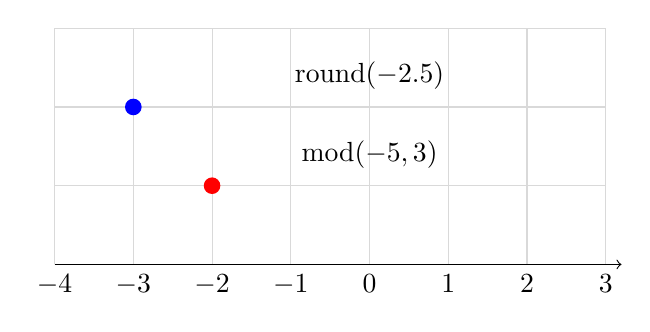
\begin{tikzpicture}
  \draw[gray!30,step=1] (-4,0) grid (3,3);
  \draw[->] (-4,0) -- (3.2,0);
  \foreach \x in {-4,-3,-2,-1,0,1,2,3}
    \node[below] at (\x,0) {$\x$};
  \fill[blue] ({round(-2.5)},2) circle (3pt);
  \fill[red] ({mod(-5,3)},1) circle (3pt);
  \node at (0,2.4) {$\operatorname{round}(-2.5)$};
  \node at (0,1.4) {$\operatorname{mod}(-5,3)$};
\end{tikzpicture}
\end{document}
